\documentclass[11pt]{article}
\usepackage{graphicx}

\topmargin 0.0cm
\oddsidemargin 0.2cm
\textwidth 16cm 
\textheight 21cm
\footskip 1.0cm

\title{Assignment Reproducible Research} 

\author
{Aleksandr Shevchenko\\
\\
\normalsize{Skolkovo Institute of Science and Technology}\\
\\
\normalsize{E-mail:  alexmtcore@gmail.com}
}

\date{}

\begin{document} 

\maketitle 

\newpage

\section{Problem setting}

The goal is to verifiy the following claim. Given the actual risk induced by Hamming distance loss function (e.g. sequence tagging tasks) and the surrogate loss function that
belongs to the family of Fenchel-Young losses, we should validate that the value of lower bound for the calibration function in this case is proportional to
$\frac{1}{T}$, where $T$ is lenght of input sequence. To confirm this we can numericaly solve the optimization problem which arises in lower bound computation for different values
of $T$ and inspect whether the relationship is correct.


\section{Experimental Validation}

In this section we present numerical validation of aforementioned claim. From the plot below it can be seen to some extent that lower bound is indeed inversely proportional to the length of
sequence $T$.

\begin{figure}[ht]
    \centering
    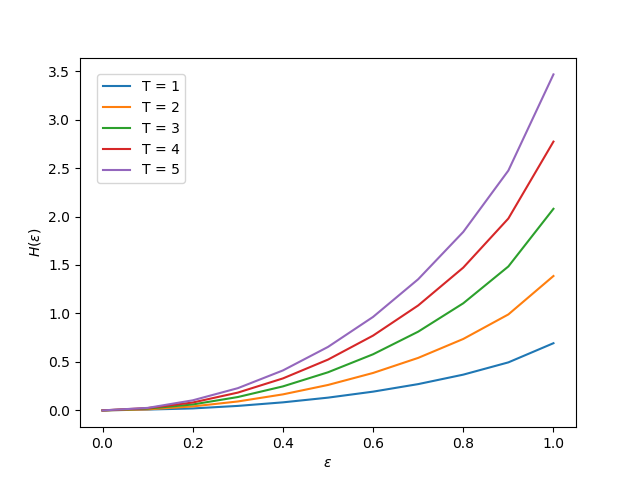
\includegraphics[width=\textwidth]{figs/comparison}
    \caption{The depence of lower bound on descrepancy $\varepsilon$ for different values of $T$.}
\end{figure}

\end{document}